\clearpage\begingroup
\newfontfamily\HeliometerGreek{STIXTwoMath-Regular.otf}
\providecommand{\ObsSec}[2]{#1\mathord{\overset{\mathrm{s}}{,}}#2}
\providecommand{\ObsArc}[2]{#1\mathord{\overset{\prime\prime}{,}}#2}
\providecommand{\ObsJupiter}{\mathord{\tikz[baseline=-.1ex,x=1em,y=1em,line width=.045em]{
  \draw (.02,.48) .. controls (.04,.70) and (.33,.69) .. (.31,.46) .. controls (.29,.29) and (.14,.19) .. (.02,.13)--(.49,.13);
  \draw (.37,.64)--(.37,-.06);}}}
\providecommand{\ObsVesta}{\mathord{\tikz[baseline=-.1ex,x=1em,y=1em,line width=.045em]{
  \draw (.04,.02) rectangle (.40,.38);
  \draw (.22,.38)--(.22,.48) (.12,.63)--(.22,.48)--(.32,.63);}}}

\SourceLeaf{295}\NoSourceHead
\begin{center}{\Large [ÜBER DAS HELIOMETER.]}\par\bigskip
{\large\textls[140]{BRIEFWECHSEL.}}\par\medskip
\textsc{Gauss} an \textsc{Gerling}, Göttingen, 17. Junius 1814.\end{center}
\noindent\hspace*{\parindent}\mbox{. . . . . .}\quad Die Art, wie unser Heliometer das Repetiren bewirkt, ist äusserst einfach. Die Hauptsache ist, dass beide Objectivhälften für sich beweglich sind; nur die eine Hälfte gibt aber eine Ablesung, diese heisse $A$, die andere $B$. Jedes Halbobjectiv macht von jedem Objecte ein Bild. Die Objecte seien 1, 2, so habe ich vier Bilder $A_1$, $A_2$, $B_1$, $B_2$. Ich bringe erst (gleichviel auf welche Art) $A_1$ mit $B_2$ in Berührung und lese ab; dann bringe ich durch Bewegung von $A$, $A_2$ mit $B_1$ in Berührung und lese wieder ab, so gibt der Unterschied den doppelten Winkel; jetzt lasse ich $A$ ruhen und bringe durch Bewegung von $B$ wieder $A_1$ mit $B_2$ in Berührung, dann wieder durch Bewegung von $A$, $A_2$ mit $B_1$ und lese wieder ab; auf diese Weise erhalte ich das vierfache etc.; beide Objectivhälften bewegen sich hiebei immer wechselsweise in einerlei Sinn und die Repetition kann so weit getrieben werden als die Grösse der Scale (die von der Weite des Rohrs abhängt und etwa $1^0 30'$ bis $1^0 35'$ beträgt) erlaubt. Da der Mittelpunkt des Oculars hiebei immer mit den Mittelpunkten von $A$, $B$ ein gleichschenklichtes Dreieck machen muss, so ist das Ocular selbst beweglich und kann mit Hülfe einer Scale immer schnell und scharf gestellt werden. Uebrigens werden aber die Beobachtungen erst dann ihren vollen Werth erhalten, wenn der Heliometer eine bessere Aufstellung hat; ich habe in München ein \textls[120]{parallatisches} Stativ bestellt, wodurch ich im Stande sein werde, helle und schwache Gegenstände bei Nacht und bei Tage leicht aufzufinden, auch wie ich hoffe
\clearpage\SourceLeaf{296}\HistoricalHead{291}{R}{ÜBER DAS HELIOMETER.}
\noindent den Positionswinkel unmittelbar zu messen, ein Vortheil, der bei der gewöhnlichen Aufstellung wegfällt. Die vier Vergrösserungen schätze ich auf 50, 70, 100, 150mal. Seit einigen Tagen beobachte ich einen sehr kleinen Sonnenfleck (nur ein Paar Secunden gross), ich hoffe, dass \textsc{Nicolai} ihn zugleich am P[assagen]-I[nstrument] beobachten wird; dann werden sich gute Resultate ergeben. Ich dachte ihn zugleich am Quadranten zu beobachten, allein es ist nur an Einem Mittage heiter gewesen, und da zeigte das elende Fernrohr desselben den Fleck beinahe gar nicht; auch ist die Zeit beinahe zu kurz für Einen Beobachter, beide Ränder und den Flecken zu nehmen und sechsfach abzulesen.\quad\mbox{. . . . . .}
\begin{center}\small\rule{.94\textwidth}{.35pt}\par
[\textsc{Wilhelm Olbers}, Sein Leben und seine Werke, II 1, Berlin 1900, S. 555. 586. 592.]\par
\rule{.94\textwidth}{.35pt}\end{center}
\begin{center}\textsc{Gauss} an \textsc{Olbers}, Göttingen, 7. Juli 1814.\end{center}
\noindent\hspace*{\parindent}\mbox{. . . . . .}\quad Mein Heliometer gibt die Rotation der Objektive nur in Graden an; ein geübtes Auge fehlt aber beim Schätzen wohl nicht leicht über $3'$, und das gibt erst bei einer Distanz von $19'$ einen Fehler von $1''$\mbox{. . . . . .}\quad Sonst denke ich die Declinationen künftig noch auf eine andre Art zu bestimmen. Ich gebe den Objectiven eine solche Stellung, dass ihre Bewegung in der Richtung eines Stundenkreises geschieht (wie es auch bei einem Faden wird sein müssen), entferne sie ungefähr um den Declinationsunterschied und bediene mich dann des Feldes als Kreismikrometer. Da ich sodann die beiden Objecte sehr nahe an Einem Rande durchgehen lassen kann, so erhalte ich, wie Sie wissen, den Declinationsunterschied, oder vielmehr die Correction dessen, was der Hel[iometer] unmittelbar angibt, mit grosser Schärfe. — Von Doppelsternen habe ich nur einen, {\HeliometerGreek β} Scorpii, erst einmal beobachtet, ich fand den Abstand $\ObsArc{13}{6}$.\quad\mbox{. . . . . .}
\begin{center}\textsc{Gauss} an \textsc{Olbers}, Göttingen, 3. April 1815.\end{center}
\noindent\hspace*{\parindent}\mbox{. . . . . .}\quad Die \textsc{Fraunhofer}schen Heliometer werden noch neue theoretisch-dioptrische Untersuchungen veranlassen, wobei noch ganz besondere Schwierigkeiten Statt finden. Da diese Instrumente bis $1\frac23$ Grad \mbox{. . . .}\ messen, und es selbst sehr wichtig sein wird, aus grossen Winkeln den Werth der
\HistoricalFoot{}{$37^{\ast}$}
\clearpage\SourceLeaf{297}\HistoricalHead{292}{L}{PRAKTISCHE UND SPHÄRISCHE ASTRONOMIE. BRIEFWECHSEL.}
\noindent Scale abzuleiten, so kommt der Umstand in Betracht, dass nach aller Strenge die Verschiebung des Objectivs dem Winkel nicht proportional ist. Soll man nun die Tangente der Hälfte, den Sinus der Hälfte oder noch etwas anderes nehmen? Das soll billig theoretisch entschieden werden, aber hier eben ist nun die Schwierigkeit. Wohin soll man eigentlich das Bild setzen von Strahlen, die nicht parallel mit der Axe auf ein Objectiv fallen? Ich denke mir einen Hauptstrahl, der auf die Mitte des Objectivs $C$ (geneigt gegen die Axe) fällt. Die Ebene durch den Strahl und die Axe gehe durch $CD$, und $D$ sei dem $C$ unendlich nahe, so kann man allerdings den Punkt bestimmen, wo die auf $C$ und $D$ fallenden Parallelstrahlen sich schneiden, und wenn das Objectiv nach richtigen Principien gearbeitet ist, d. i. so, dass die sogenannte Abweichung wegen der Kugelgestalt gehoben ist, so werden auch alle übrigen Parallelstrahlen, die in derselben Ebene durch $CD$ auffallen, sich sehr nahe in eben dem Punkte vereinigen.
\begin{center}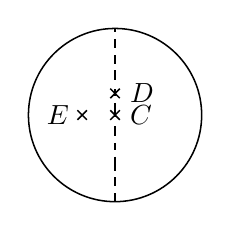
\begin{tikzpicture}[x=1.1cm,y=1.1cm,line width=.55pt]
\draw (0,0) circle[radius=1];
\draw (0,1)--(0,.96) (0,.88)--(0,.77) (0,.69)--(0,.59)
 (0,.52)--(0,.40) (0,.30)--(0,.22) (0,.14)--(0,-.02)
 (0,-.13)--(0,-.24) (0,-.32)--(0,-.40) (0,-.48)--(0,-.65)
 (0,-.72)--(0,-.82) (0,-.90)--(0,-1);
\draw (-.055,.195)--(.055,.305) (-.055,.305)--(.055,.195);
\draw (-.055,-.055)--(.055,.055) (-.055,.055)--(.055,-.055);
\draw (-.435,-.055)--(-.325,.055) (-.435,.055)--(-.325,-.055);
\node[anchor=west,inner sep=2pt] at (.10,.25) {$D$};
\node[anchor=west,inner sep=2pt] at (.10,0) {$C$};
\node[anchor=east,inner sep=2pt] at (-.46,0) {$E$};
\end{tikzpicture}
\end{center}
\noindent Allein dasselbe darf man nicht von den Parallelstrahlen behaupten, die seitwärts (im $E$) auffallen; mit einem Wort, der Brennpunkt, aus $C$ und $D$ bestimmt, wird ein anderer sein, als aus $C$ und $E$ bestimmt. Beträchtlich wird der Unterschied freilich nicht sein, aber allgemein zu reden von derselben Ordnung, wie der Unterschied zwischen Bogen und Sinus. Vielleicht wird man auf 3erlei verschiedene Art rechnen müssen, je nachdem die Objecte sind, die man zusammenbringt: anders wenn zwei Punkte einander decken sollen (wie Sterne und kleine Löcher etc.), anders wenn zwei Linien der Länge nach sich berühren (wie die Sonnenränder), anders wenn zwei Linien sich bloss an den Endpunkten berühren. Von einer andern Seite betrachtet, scheint es mir doch, als ob man den Brennpunkt immer aus $C$ und $D$ bestimmen müsse, ohne sich um $E$ zu bekümmern. Ich habe mir zum Behuf dieser Rechnung von \textsc{Fraunhofer} die vier Halbmesser der Glasflächen ausgebeten.\quad\mbox{. . . . . .}
\begin{center}\textsc{Gauss} an \textsc{Olbers}, Göttingen, 29. Mai 1815.\end{center}
\noindent\hspace*{\parindent}\mbox{. . . . . .}\quad Mein parallatisches Stativ ist denn endlich angekommen. Es ist ein treffliches Kunstwerk, freilich etwas complicirt. Es hat mir viel Vergnügen gemacht, für die mannichfaltigen Berichtigungen dabei Methoden auszusinnen.
\clearpage\SourceLeaf{298}\HistoricalHead{293}{R}{ÜBER DAS HELIOMETER.}
\noindent Bisher habe ich sie aber erst im Groben gemacht, da in dem neuen Ocular erst Spinnenfäden eingezogen werden müssen, woran es bisher gefehlt hat.\quad\mbox{. . . . .}\quad Aber auch bei der frühern groben Berichtigung fand ich die Venus sogleich am Tage. Sehen Sie zur Probe die Messung des Venusdurchmessers am 16. Mai Nachmittags
\begin{center}\renewcommand{\arraystretch}{1.15}\begin{tabular}{clrrc}
Abfahrtspunct&Partes&50&$56{,}4$&1fach\\
2fach&&50&$13{,}6$&$21{,}40=\ObsArc{12}{08}$\\
4fach&&49&$71{,}1$&$21{,}32=12{,}04$\\
6fach&&49&$30{,}0$&$21{,}07=11{,}90$\\
8fach&&48&$88{,}6$&$20{,}97=11{,}84$\\
10fach&&48&$47{,}6$&$20{,}88=11{,}79$.
\end{tabular}\end{center}
\noindent\hspace*{\parindent}Die theoretische Schwierigkeit, wovon ich Ihnen in meinem letzten Briefe schrieb, hat insofern eine praktische Wichtigkeit, als ich gern den genauen Werth der Scale aus einem so grossen Winkel, als das Instrument nur fasst, bestimmen möchte. Ich denke dabei in Zukunft etwa folgendes Verfahren anzuwenden. Ich lasse etwa 6 Stangen $A$, $B$, $C$ etc. ausstecken
\begin{center}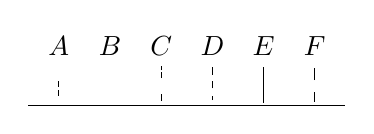
\begin{tikzpicture}[x=.65cm,y=.65cm,line width=.35pt]
\draw (-.60,0)--(5.60,0);
\draw (0,.18)--(0,.30) (0,.36)--(0,.48);
\draw (2,.08)--(2,.22) (2,.53)--(2,.65) (2,.68)--(2,.76);
\draw (3,.10)--(3,.18) (3,.33)--(3,.48) (3,.60)--(3,.74);
\draw (4,.05)--(4,.74);
\draw (5,.07)--(5,.25) (5,.49)--(5,.73);
\node at (0,1.15) {$A$};\node at (1,1.15) {$B$};
\node at (2,1.15) {$C$};\node at (3,1.15) {$D$};
\node at (4,1.15) {$E$};\node at (5,1.15) {$F$};
\end{tikzpicture}
\end{center}
\noindent so dass $AB$, $BC$, $CD$ etc. ungefähr unter sich gleich sind und etwa einen Winkel von $1\frac12$ Grad machen, messe die Entfernungen einzeln mit dem Heliometer und $AF$ collective mit dem Kreise durch Repetition. Es fehlt nur noch an einem schicklichen von der Sternwarte aus sichtbaren Platze.\quad\mbox{. . . . . .}
\begin{center}BEMERKUNGEN.\end{center}
\begingroup\small
\noindent\hspace*{\parindent}Im Juni 1814 erhielt die Göttinger Sternwarte ein \textsc{Fraunhofer}sches Heliometer, von dem \textsc{Gauss} jedoch keinen häufigen Gebrauch gemacht hat. Auf der alten Sternwarte fehlte anfangs ein brauchbares Stativ, und auf der neuen Sternwarte fand sich zunächst keine günstige Gelegenheit zur Aufstellung des Instruments. Weiterhin war \textsc{Gauss}' Zeit durch andere Arbeiten vollständig in Anspruch genommen. Näheres darüber findet man in dem Aufsatz über \textsc{Gauss}' astronomische Arbeiten, Werke XI 2.
\begin{flushright}\textsc{Brendel}.\end{flushright}
\endgroup
\begin{center}\rule{.31\textwidth}{.35pt}\end{center}
\clearpage\endgroup
